\documentclass{article}
\usepackage[utf8]{inputenc}
\usepackage{listings}
\usepackage{xcolor}
\usepackage{graphicx}
\usepackage{float}

\title{Computer Architecture Lab-5: Pipeline Stall Detector}
\author{Pradeep Mundlik}
\date{\today}

\begin{document}

\maketitle

\section{Introduction}

The objective of this lab exercise is to implement a basic pipeline hazard detection and data forwarding mechanism in assembly code. The code provided reads an assembly program from an input file and analyzes it to identify potential hazards and insert "NOP" (No-Operation) instructions to resolve them. Two approaches are implemented: one without data forwarding and one with data forwarding.

\section{Code Explanation}

\subsection{Input Reading}

The code starts by reading an assembly program from an input file named "input.txt" and stores it in a vector called \texttt{program}. Each line of the input file represents an assembly instruction.

\subsection{Instruction Parsing}

The \texttt{parseInstruction} function extracts the instruction name, destination registers, and source registers from a given assembly instruction. It handles various assembly instruction formats, including load and store instructions.

\subsection{Adding NOPs (assuming no data forwarding and hazard detection)}

The \texttt{addNops} function analyzes the assembly program and detects hazards caused by dependencies between instructions. If a source register in an instruction depends on the result of a previous instruction, "NOP" instructions are inserted to resolve the hazard. The code ensures that "NOP" instructions are added in the correct positions in the program.

\subsection{Adding NOPs (with data forwarding and hazard detection)}

The \texttt{addNopsDataForwarding} function implements data forwarding to resolve hazards. It checks if a load instruction (e.g., \texttt{ld}) is followed by an instruction that depends on the load result. If such a dependency exists, a "NOP" instruction is inserted to stall the pipeline.

\section{Testing Code}

The code is executed with and without data forwarding, and the modified assembly programs are displayed along with the total number of clock cycles required for execution. The results of both approaches are presented as follows:

\subsection{Test Case: Sample Input and Output}

\begin{verbatim}
Sample Input:
    add x14, x12, x11
    add x15, x14, x12
    ld x13, 8(x13)
    ld x12, 0(x14)
    and x13, x15, x13
    ld x11, 4(x13)
    sd x13, 0(x15)
Output:
    Without data forwading: 

    add x14, x12, x11
    NOP
    NOP
    add x15, x14, x12
    ld x13, 8(x13)
    ld x12, 0(x14)
    NOP
    and x13, x15, x13
    NOP
    NOP
    ld x11, 4(x13)
    sd x13, 0(x15)
    Total: 16 cycles

    With data forwading: 

    add x14, x12, x11
    add x15, x14, x12
    ld x13, 8(x13)
    ld x12, 0(x14)
    and x13, x15, x13
    ld x11, 4(x13)
    sd x13, 0(x15)
    Total: 11 cycles

\end{verbatim}
\begin{figure}[H]{\centering}
    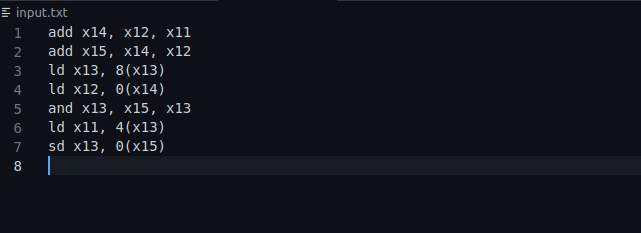
\includegraphics[width=\textwidth]{input.png}
    \caption[short]{Input}
\end{figure}
\begin{figure}[H]
    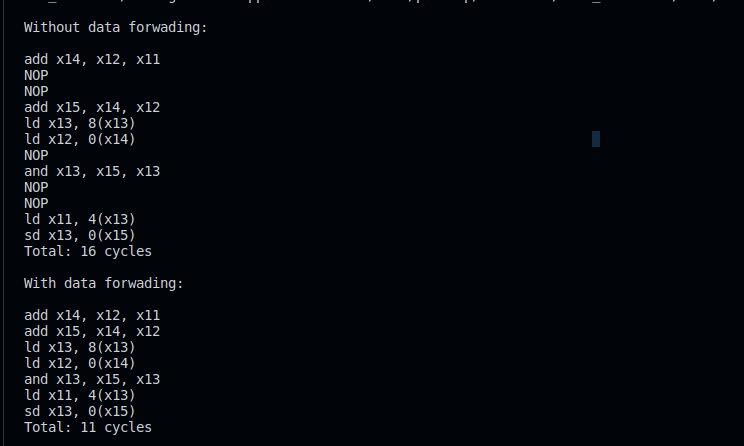
\includegraphics[width=\textwidth]{output.png}
    \caption[short]{Output}
\end{figure}
\end{document}
   